% Options for packages loaded elsewhere
\PassOptionsToPackage{unicode}{hyperref}
\PassOptionsToPackage{hyphens}{url}
%
\documentclass[
]{article}
\usepackage{amsmath,amssymb}
\usepackage{iftex}
\ifPDFTeX
  \usepackage[T1]{fontenc}
  \usepackage[utf8]{inputenc}
  \usepackage{textcomp} % provide euro and other symbols
\else % if luatex or xetex
  \usepackage{unicode-math} % this also loads fontspec
  \defaultfontfeatures{Scale=MatchLowercase}
  \defaultfontfeatures[\rmfamily]{Ligatures=TeX,Scale=1}
\fi
\usepackage{lmodern}
\ifPDFTeX\else
  % xetex/luatex font selection
\fi
% Use upquote if available, for straight quotes in verbatim environments
\IfFileExists{upquote.sty}{\usepackage{upquote}}{}
\IfFileExists{microtype.sty}{% use microtype if available
  \usepackage[]{microtype}
  \UseMicrotypeSet[protrusion]{basicmath} % disable protrusion for tt fonts
}{}
\makeatletter
\@ifundefined{KOMAClassName}{% if non-KOMA class
  \IfFileExists{parskip.sty}{%
    \usepackage{parskip}
  }{% else
    \setlength{\parindent}{0pt}
    \setlength{\parskip}{6pt plus 2pt minus 1pt}}
}{% if KOMA class
  \KOMAoptions{parskip=half}}
\makeatother
\usepackage{xcolor}
\usepackage[margin=1in]{geometry}
\usepackage{color}
\usepackage{fancyvrb}
\newcommand{\VerbBar}{|}
\newcommand{\VERB}{\Verb[commandchars=\\\{\}]}
\DefineVerbatimEnvironment{Highlighting}{Verbatim}{commandchars=\\\{\}}
% Add ',fontsize=\small' for more characters per line
\usepackage{framed}
\definecolor{shadecolor}{RGB}{248,248,248}
\newenvironment{Shaded}{\begin{snugshade}}{\end{snugshade}}
\newcommand{\AlertTok}[1]{\textcolor[rgb]{0.94,0.16,0.16}{#1}}
\newcommand{\AnnotationTok}[1]{\textcolor[rgb]{0.56,0.35,0.01}{\textbf{\textit{#1}}}}
\newcommand{\AttributeTok}[1]{\textcolor[rgb]{0.13,0.29,0.53}{#1}}
\newcommand{\BaseNTok}[1]{\textcolor[rgb]{0.00,0.00,0.81}{#1}}
\newcommand{\BuiltInTok}[1]{#1}
\newcommand{\CharTok}[1]{\textcolor[rgb]{0.31,0.60,0.02}{#1}}
\newcommand{\CommentTok}[1]{\textcolor[rgb]{0.56,0.35,0.01}{\textit{#1}}}
\newcommand{\CommentVarTok}[1]{\textcolor[rgb]{0.56,0.35,0.01}{\textbf{\textit{#1}}}}
\newcommand{\ConstantTok}[1]{\textcolor[rgb]{0.56,0.35,0.01}{#1}}
\newcommand{\ControlFlowTok}[1]{\textcolor[rgb]{0.13,0.29,0.53}{\textbf{#1}}}
\newcommand{\DataTypeTok}[1]{\textcolor[rgb]{0.13,0.29,0.53}{#1}}
\newcommand{\DecValTok}[1]{\textcolor[rgb]{0.00,0.00,0.81}{#1}}
\newcommand{\DocumentationTok}[1]{\textcolor[rgb]{0.56,0.35,0.01}{\textbf{\textit{#1}}}}
\newcommand{\ErrorTok}[1]{\textcolor[rgb]{0.64,0.00,0.00}{\textbf{#1}}}
\newcommand{\ExtensionTok}[1]{#1}
\newcommand{\FloatTok}[1]{\textcolor[rgb]{0.00,0.00,0.81}{#1}}
\newcommand{\FunctionTok}[1]{\textcolor[rgb]{0.13,0.29,0.53}{\textbf{#1}}}
\newcommand{\ImportTok}[1]{#1}
\newcommand{\InformationTok}[1]{\textcolor[rgb]{0.56,0.35,0.01}{\textbf{\textit{#1}}}}
\newcommand{\KeywordTok}[1]{\textcolor[rgb]{0.13,0.29,0.53}{\textbf{#1}}}
\newcommand{\NormalTok}[1]{#1}
\newcommand{\OperatorTok}[1]{\textcolor[rgb]{0.81,0.36,0.00}{\textbf{#1}}}
\newcommand{\OtherTok}[1]{\textcolor[rgb]{0.56,0.35,0.01}{#1}}
\newcommand{\PreprocessorTok}[1]{\textcolor[rgb]{0.56,0.35,0.01}{\textit{#1}}}
\newcommand{\RegionMarkerTok}[1]{#1}
\newcommand{\SpecialCharTok}[1]{\textcolor[rgb]{0.81,0.36,0.00}{\textbf{#1}}}
\newcommand{\SpecialStringTok}[1]{\textcolor[rgb]{0.31,0.60,0.02}{#1}}
\newcommand{\StringTok}[1]{\textcolor[rgb]{0.31,0.60,0.02}{#1}}
\newcommand{\VariableTok}[1]{\textcolor[rgb]{0.00,0.00,0.00}{#1}}
\newcommand{\VerbatimStringTok}[1]{\textcolor[rgb]{0.31,0.60,0.02}{#1}}
\newcommand{\WarningTok}[1]{\textcolor[rgb]{0.56,0.35,0.01}{\textbf{\textit{#1}}}}
\usepackage{graphicx}
\makeatletter
\def\maxwidth{\ifdim\Gin@nat@width>\linewidth\linewidth\else\Gin@nat@width\fi}
\def\maxheight{\ifdim\Gin@nat@height>\textheight\textheight\else\Gin@nat@height\fi}
\makeatother
% Scale images if necessary, so that they will not overflow the page
% margins by default, and it is still possible to overwrite the defaults
% using explicit options in \includegraphics[width, height, ...]{}
\setkeys{Gin}{width=\maxwidth,height=\maxheight,keepaspectratio}
% Set default figure placement to htbp
\makeatletter
\def\fps@figure{htbp}
\makeatother
\setlength{\emergencystretch}{3em} % prevent overfull lines
\providecommand{\tightlist}{%
  \setlength{\itemsep}{0pt}\setlength{\parskip}{0pt}}
\setcounter{secnumdepth}{-\maxdimen} % remove section numbering
\ifLuaTeX
  \usepackage{selnolig}  % disable illegal ligatures
\fi
\usepackage{bookmark}
\IfFileExists{xurl.sty}{\usepackage{xurl}}{} % add URL line breaks if available
\urlstyle{same}
\hypersetup{
  pdftitle={Data 602 - Project},
  pdfauthor={Josh Brauner, Raahim Salman, Ze Yu},
  hidelinks,
  pdfcreator={LaTeX via pandoc}}

\title{Data 602 - Project}
\author{Josh Brauner, Raahim Salman, Ze Yu}
\date{Feburary 14th, 2024}

\begin{document}
\maketitle

\section{Part 1}\label{part-1}

\subsection{Data Wrangling}\label{data-wrangling}

In the initial phase of our project, the primary goal is to prepare the
dataset for analysis. This preparation involves loading the data and
then removing data points that could potentially skew or bias our
results. Specifically, the dataset encompasses annual home run rates
(home runs per at bat) for Barry Bonds, covering several seasons. Per
the project's guidelines, it's imperative to exclude the 2001
season---the year Barry Bonds hit a record 73 home runs---from our
dataset before proceeding with any further analysis. The rationale
behind excluding this particular season is rooted in its outlier status
within the scope of our investigation, possibly due to factors such as
intentional walks, which are not reflective of the typical performance
trends we aim to analyze.

\begin{Shaded}
\begin{Highlighting}[]
\NormalTok{bonds\_data }\OtherTok{\textless{}{-}} \FunctionTok{read.csv}\NormalTok{(}\StringTok{"/Users/rs/MDataSci/data601/project/bondsdata.csv"}\NormalTok{)}
\NormalTok{bonds\_data\_filtered }\OtherTok{\textless{}{-}} \FunctionTok{subset}\NormalTok{(bonds\_data, season }\SpecialCharTok{!=} \DecValTok{2001}\NormalTok{)}
\FunctionTok{tail}\NormalTok{(bonds\_data\_filtered)}
\end{Highlighting}
\end{Shaded}

\begin{verbatim}
##    season     hrat
## 9    1995 0.065217
## 10   1996 0.081238
## 11   1997 0.075188
## 12   1998 0.067029
## 13   1999 0.095775
## 14   2000 0.102083
\end{verbatim}

The removal of the 2001 season data point is a critical step in ensuring
a more accurate and unbiased evaluation of Bonds' performance trends
over the years leading up to this extraordinary season. By focusing on
the years preceding 2001, we aim to construct a statistical model that
predicts Bonds' home run rates without the influence of this anomalous
year. This approach is intended to provide a clearer perspective on his
performance trajectory, allowing us to assess whether there is evidence
of an unusual improvement that could be attributed to external factors,
such as the speculated use of steroids.

\subsection{Model Building}\label{model-building}

The statistical model we plan to build,
\(HRAT_{i} = A + B \times Year_{i} + e_{i}\), where \(HRAT_{i}\)
represents the home run rate in year \(i\), and \(Year_{i}\) denotes the
year of the season, is designed to elucidate the relationship between
time (years) and Bonds' home run rates. Through quantifying the trend
over the specified years, this linear regression model serves as a tool
for analyzing potential significant deviations in performance. Such
deviations, if present, could align with steroid use, under the premise
that such use would manifest as an atypical increase in home run rates.

\begin{Shaded}
\begin{Highlighting}[]
\NormalTok{model }\OtherTok{\textless{}{-}} \FunctionTok{lm}\NormalTok{(hrat }\SpecialCharTok{\textasciitilde{}}\NormalTok{ season, }\AttributeTok{data =}\NormalTok{ bonds\_data\_filtered)}
\NormalTok{model}\SpecialCharTok{$}\NormalTok{coef}
\end{Highlighting}
\end{Shaded}

\begin{verbatim}
##  (Intercept)       season 
## -7.992499290  0.004044169
\end{verbatim}

The linear regression equation representing the model is
\(\hat{HRAT_{i}} = -7.992 + 0.004 \times Year_{i}\).

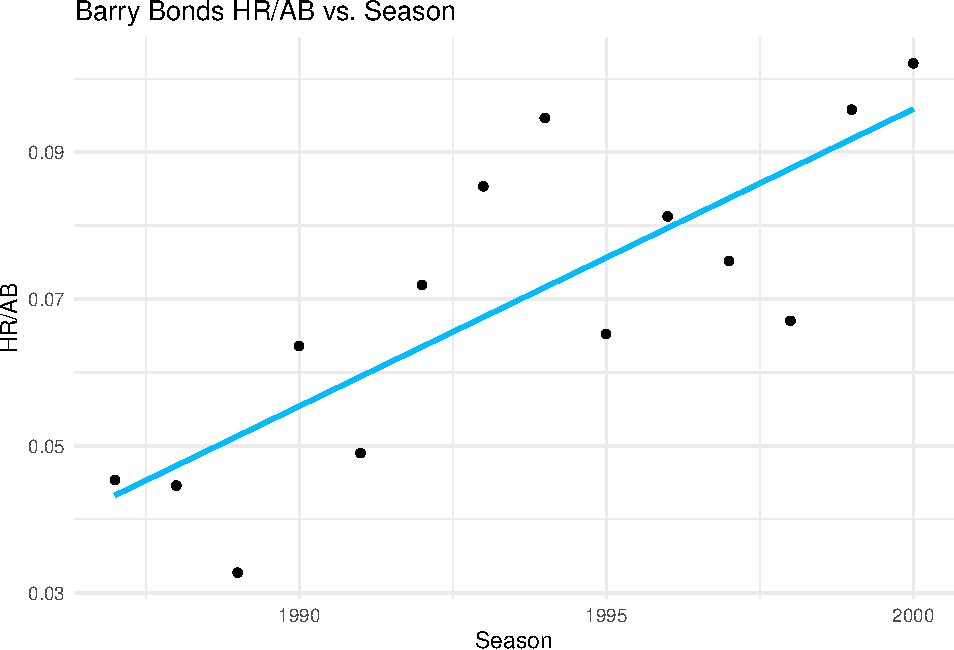
\includegraphics{602_project_files/figure-latex/unnamed-chunk-4-1.pdf}

Importantly, to ensure the integrity of the conclusions drawn from this
model, we will verify the assumptions underlying linear regression
analysis, including linearity, independence of errors, homoscedasticity
(constant variance of errors), and normality of error terms. These
checks are fundamental to confirming that our model is accurately
specified and that the inferences and predictions derived from it are
reliable.

\subsection{Model Assumption and
Validation}\label{model-assumption-and-validation}

\textbf{\emph{Correlation Coefficient Check}}:

\begin{Shaded}
\begin{Highlighting}[]
\FunctionTok{cor}\NormalTok{(bonds\_data\_filtered}\SpecialCharTok{$}\NormalTok{season, bonds\_data\_filtered}\SpecialCharTok{$}\NormalTok{hrat)}
\end{Highlighting}
\end{Shaded}

\begin{verbatim}
## [1] 0.7981544
\end{verbatim}

A correlation coefficient of 0.7981544 indicates a strong positive
linear relationship between the year and the home runs per at bat
(HR/AB) for Barry Bonds, excluding the 2001 season.

\textbf{\emph{Significance of Coefficient Estimates}}

In the context of analyzing the significance of the coefficient estimate
for the year in predicting home runs per at bat (HR/AB) for Barry Bonds
(excluding the 2001 season), we can formulate the null hypothesis
(\(H_0\)) and the alternative hypothesis (\(H_1\)) as follows, with an
alpha level (\(\alpha\)) of 0.05:

Null hypothesis: \(H_{0}: \beta_{1} = 0\), \(H_{0}: \beta_{0} = 0\)

Alternative hypothesis: \(H_{A}: \beta_{1} \neq 0\),
\(H_{A}: \beta_{0} \neq 0\)

\begin{Shaded}
\begin{Highlighting}[]
\FunctionTok{summary}\NormalTok{(model)}
\end{Highlighting}
\end{Shaded}

\begin{verbatim}
## 
## Call:
## lm(formula = hrat ~ season, data = bonds_data_filtered)
## 
## Residuals:
##       Min        1Q    Median        3Q       Max 
## -0.020722 -0.009931  0.001841  0.007701  0.023055 
## 
## Coefficients:
##               Estimate Std. Error t value Pr(>|t|)    
## (Intercept) -7.9924993  1.7566775  -4.550 0.000666 ***
## season       0.0040442  0.0008812   4.589 0.000622 ***
## ---
## Signif. codes:  0 '***' 0.001 '**' 0.01 '*' 0.05 '.' 0.1 ' ' 1
## 
## Residual standard error: 0.01329 on 12 degrees of freedom
## Multiple R-squared:  0.6371, Adjusted R-squared:  0.6068 
## F-statistic: 21.06 on 1 and 12 DF,  p-value: 0.0006222
\end{verbatim}

\begin{Shaded}
\begin{Highlighting}[]
\FunctionTok{coef}\NormalTok{(}\FunctionTok{summary}\NormalTok{(model))[, }\StringTok{"t value"}\NormalTok{]}
\end{Highlighting}
\end{Shaded}

\begin{verbatim}
## (Intercept)      season 
##   -4.549782    4.589384
\end{verbatim}

\begin{Shaded}
\begin{Highlighting}[]
\FunctionTok{coef}\NormalTok{(}\FunctionTok{summary}\NormalTok{(model))[, }\StringTok{"Pr(\textgreater{}|t|)"}\NormalTok{]}
\end{Highlighting}
\end{Shaded}

\begin{verbatim}
##  (Intercept)       season 
## 0.0006664296 0.0006222474
\end{verbatim}

\subsubsection{Intercept}\label{intercept}

\begin{itemize}
\tightlist
\item
  \textbf{t-value for Intercept}: -4.549782
\item
  \textbf{p-value for Intercept}: 0.0006664296
\end{itemize}

The intercept's t-value is significantly negative, and the corresponding
p-value is much less than the alpha level of 0.05. This statistically
significant result suggests that the intercept is significantly
different from zero. Therefore we reject the null hypothesis
\(H_0: B_{0} = 0\) in favor of the alternative hypothesis
\(H_1: B_{0} \neq 0\)\$.

\subsubsection{Season}\label{season}

\begin{itemize}
\tightlist
\item
  \textbf{t-value for Season}: 4.589384
\item
  \textbf{p-value for Season}: 0.0006222474
\end{itemize}

The t-value for the year coefficient is significantly positive,
indicating a positive relationship between the year and HR/AB ratio for
Barry Bonds in the dataset analyzed. The p-value associated with this
t-value is much less than 0.05, strongly suggesting that we reject the
null hypothesis \(H_0: B_{1} = 0\) in favor of the alternative
hypothesis \(H_1: B_{1} \neq 0\).

\subsubsection{Implications}\label{implications}

The statistical analysis of the year's coefficient reveals that there is
a significant linear relationship between the year and the HR/AB ratio.
This means that the year significantly predicts the HR/AB ratio for
Barry Bonds in the years leading up to 2001, excluding the 2001 season
itself. The positive t-value indicates that as the year increases, so
does the HR/AB ratio, suggesting an improvement in Bonds' performance in
hitting home runs per at-bat attempt over time.

Given the alpha level of 0.05 and the very low p-values obtained for
both the intercept and the year coefficient, our analysis provides
strong statistical evidence to support the conclusion that there was a
significant trend in Barry Bonds' home run rates per at-bat over the
years analyzed.

The R-squared value of 0.6371 in your linear regression model indicates
that approximately 63.71\% of the variance in the dependent variable is
explained by the independent variable.

\textbf{Residual Analysis}

\subsubsection{Normality of Residuals}\label{normality-of-residuals}

In our specific analysis concerning Barry Bonds' home run rates (HR/AB)
as a function of the season (year), the normality of residuals implies
that the deviations from the predicted home run rates are random and
follow a normal distribution. This condition supports the premise that
our linear model is appropriately capturing the relationship between the
year and HR/AB without systematic bias.

The evidence supporting the normality of residuals in our analysis comes
from both graphical and statistical methods:

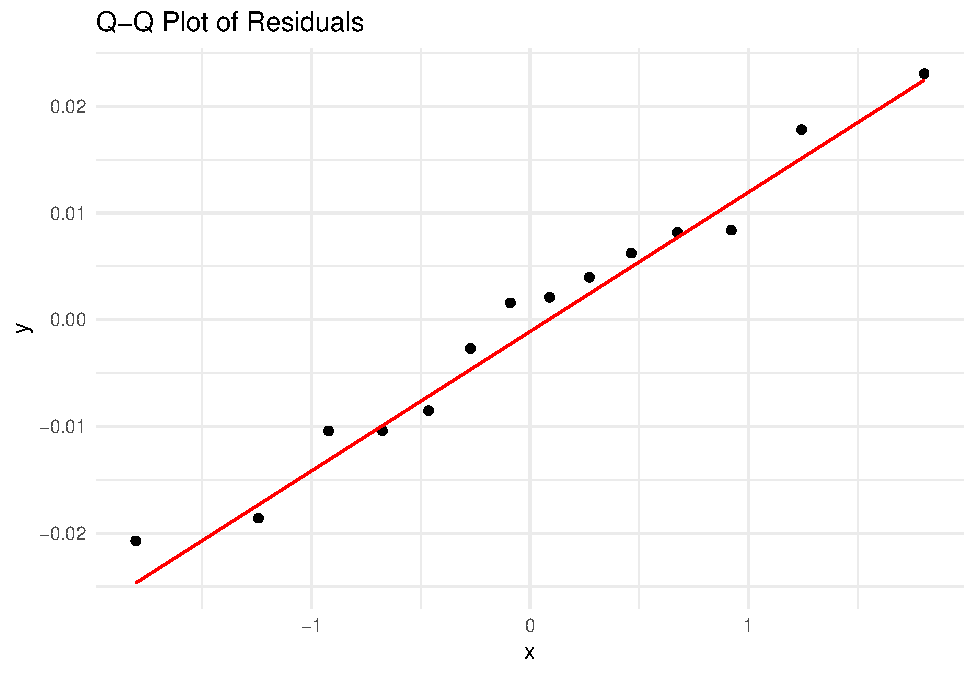
\includegraphics{602_project_files/figure-latex/unnamed-chunk-7-1.pdf}

In our case, the residuals align closely with the reference line in the
Q-Q plot, indicating that their distribution resembles a normal
distribution. This evidence suggests that the residuals from our linear
model do not deviate significantly from normality.

\begin{Shaded}
\begin{Highlighting}[]
\FunctionTok{shapiro.test}\NormalTok{(residuals)}
\end{Highlighting}
\end{Shaded}

\begin{verbatim}
## 
##  Shapiro-Wilk normality test
## 
## data:  residuals
## W = 0.97132, p-value = 0.8938
\end{verbatim}

The Shapiro-Wilk test is a statistical test designed to assess the
normality of a dataset. In our analysis, the Shapiro-Wilk test for the
residuals yields a p-value of 0.8938. Given that this p-value is
significantly greater than the conventional threshold of 0.05, we fail
to reject the null hypothesis that the residuals are normally
distributed. This statistical evidence further substantiates the claim
that the residuals of our model are normal.

\subsubsection{Homoscedasticity}\label{homoscedasticity}

The examination of homoscedasticity is a critical step in validating the
assumptions underlying a linear regression model. Homoscedasticity
refers to the condition where the residuals (the differences between
observed and predicted values) have constant variance across all levels
of the independent variable(s). This assumption ensures that the model's
predictive accuracy is uniform across the range of the independent
variable, which in this context is the season (year) for Barry Bonds'
home run rates (HR/AB).

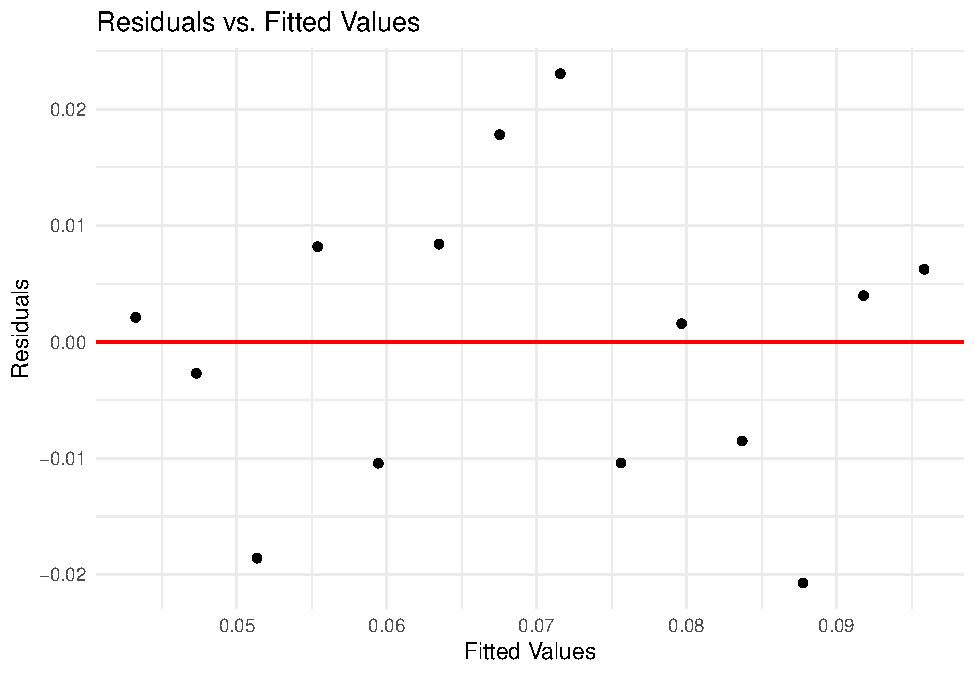
\includegraphics{602_project_files/figure-latex/unnamed-chunk-9-1.pdf}

\begin{Shaded}
\begin{Highlighting}[]
\FunctionTok{bptest}\NormalTok{(model)}
\end{Highlighting}
\end{Shaded}

\begin{verbatim}
## 
##  studentized Breusch-Pagan test
## 
## data:  model
## BP = 0.04849, df = 1, p-value = 0.8257
\end{verbatim}

The Breusch-Pagan (BP) test is a statistical procedure designed to test
for heteroscedasticity --- the presence of non-constant variance in the
error terms of a regression model. In the context of analyzing Barry
Bonds' home run rates (HR/AB) as a function of the season (year), the BP
test's p-value of 0.8257 significantly exceeds the common alpha level
threshold of 0.05. This high p-value indicates that there is
insufficient evidence to reject the null hypothesis of the BP test,
which states that the error variances are homoscedastic.

The even distribution of residuals across the predicted values, as
evidenced by the scatter plot, allows us to conclude that the condition
of homoscedasticity holds for our linear regression model. This finding
is crucial because it means that our model meets another important
assumption of linear regression, reinforcing its validity and the
reliability of its predictions and inferences.

Given that our analysis has confirmed both key assumptions of linear
regression---normality of residuals and homoscedasticity---we can assert
that our linear regression model is valid. This validity implies that
the model is well-founded and that the statistical inferences drawn from
it, such as confidence intervals and hypothesis tests on the regression
coefficients, are based on solid assumptions.

\subsection{Prediction of Home Run Rate in 2001
Season}\label{prediction-of-home-run-rate-in-2001-season}

\begin{Shaded}
\begin{Highlighting}[]
\NormalTok{new\_data }\OtherTok{\textless{}{-}} \FunctionTok{data.frame}\NormalTok{(}\AttributeTok{season =} \DecValTok{2001}\NormalTok{)}
\NormalTok{predicted\_hrab }\OtherTok{\textless{}{-}} \FunctionTok{predict}\NormalTok{(model, }\AttributeTok{newdata =}\NormalTok{ new\_data, }\AttributeTok{interval =} \StringTok{"predict"}\NormalTok{)}
\FunctionTok{print}\NormalTok{(predicted\_hrab)}
\end{Highlighting}
\end{Shaded}

\begin{verbatim}
##          fit        lwr       upr
## 1 0.09988334 0.06662845 0.1331382
\end{verbatim}

The 95\% prediction interval for Bonds' HRAT in the 2001 season, ranging
from 0.06663 to 0.13314, represents the range within which we would
expect Bonds' HRAT to fall, given the trends observed in the data from
previous seasons. The fact that Bonds' actual HRAT of 0.153400 falls
outside this interval suggests that his performance in 2001 was not only
exceptional but also statistically significant in terms of deviation
from predicted trends.

While the statistical analysis does not directly address whether Barry
Bonds was using steroids in the 2001 season, the significant discrepancy
between the predicted and actual HRATs, and the fact that the actual
HRAT lies outside the 95\% prediction interval, suggest that there were
factors influencing Bonds' performance that year beyond what could be
expected based on historical trends.

In conclusion, while our linear regression model and subsequent analysis
provide valuable insights into Barry Bonds' performance trends leading
up to the 2001 season, they also highlight an extraordinary deviation in
his 2001 performance that warrants further investigation. The
statistical evidence suggests that Bonds' HRAT in 2001 was significantly
higher than expected based on past performance, pointing to the presence
of additional factors that contributed to this anomaly.

It's important to note that statistical analysis alone cannot prove the
use of performance-enhancing substances. Such conclusions would require
corroborative evidence beyond the scope of this statistical model.
However, our analysis does underscore the exceptional nature of Bonds'
2001 season within the context of his career performance trends.

\end{document}
